\documentclass[a4paper,10.0pt,twoside]{npr}

\usepackage{multicol,graphicx,lastpage,footmisc,fancyhdr,paralist,
tabularx,array,booktabs,caption,multirow,upgreek,mathrsfs,gensymb,color}
\usepackage[fancyhdr,space,fntef,fontset=ubuntu]{ctex}
\usepackage{amssymb,bm,mathrsfs,bbm,amscd}
\usepackage{flushend,cuted}
\usepackage{refcount}
\usepackage{savesym}
\usepackage{textcomp}
\usepackage[tbtags]{amsmath}  %
\savesymbol{iint}
\usepackage{amstext} %数学宏包文本命令
\usepackage{balance} %版心底部对齐

\flushbottom      %版心底部对齐
\setcounter{section}{0}
\begin{document}
%\begin{CJK*}{GBK}{\song}{\wuhao}{\rm}

%___________________________________________________________________________________
\def\rd{{\rm d}}

\newcommand{\RM}{\ensuremath{\mathrm}}   %正体 既可用于文本模式也可用于数学模式
\newcommand{\dif}{\mathrm{d}}  %直立体d
\newcommand{\me}{\mathrm{e}}  %直立体e
\newcommand{\mi}{\mathrm{i}}  %直立体i
\newcommand{\mj}{\mathrm{j}}  %直立体j
\newcommand{\afrac}[2]{\dfrac{\,#1\,}{\,#2\,}}  %略长分数线
\newcommand{\nn}{\nonumber}  %公式无编号
\newcommand{\nt}{\noindent}
\newcommand{\OO}{~\text{。}}
\newcommand{\PP}{~\text{,}}
\newcommand{\OP}{~\text{;}}
\newcommand{\LT}{\left}
\newcommand{\RT}{\right}

%___________________________________________________________________________________

\balance
\fancypagestyle{myfoot}
{%
\fancyhf{}
\fancyhead[c]{\wuhao\song 高~等~核~物~理~实~验}
\renewcommand{\headrule}{\vskip 2pt
\hrule height0.4pt width\headwidth \vskip1pt
\hrule height0.4pt width\headwidth \vskip-1.8pt}
}%
\thispagestyle{myfoot}

%%%%%%%%%%%%%%%%%%%%%%%%%%%%%%%%%%%%%%%%%%%%%%%%%%%%%
%    奇偶页眉
%%%%%%%%%%%%%%%%%%%%%%%%%%%%%%%%%%%%%%%%%%%%%%%%%%%%%
\pagestyle{fancy}
\fancyhead{}
\fancyhead[ce]{\xiaowu\song \hspace{0.5em}高~等~核~物~理~实~验}
%\fancyhead[ro,le]{\xiaowuhao \hspace{0.5em}\textbf{\textperiodcentered}\;\thepage\;\textbf{\textperiodcentered}\hspace{0.5em}}
%\fancyhead[ce]{\xiaowu\song 粒~子~物~理~与~原~子~核~物~理~专~题~实~验}
%\fancyhead[re]{\xiaowu\song \hspace{0.5em}第\;31\;卷\hspace{0.5em}}
\fancyfoot[ce,co]{}
\renewcommand{\headrule}{\vskip 2pt
\hrule height0.4pt width\headwidth}


\setcounter{page}{001}%
\fancyhead[co]{\xiaowuhao\song  乔颢:卢瑟福散射}    %奇页页眉
\begin{center}
\title{%
\xiaoerhao \bf  %章标题为两行时改为 \exiaoer
卢瑟福散射\\[-5mm]}
\maketitle
\large \fs
乔颢$^{^1}$\\[2mm]

\xiaowu \song
1. 北京大学物理学院,海淀区 北京 100871;\\[4mm]

 
\footnotetext[0]{{\bf 作者简介:}~~\begin{minipage}[t][4.2mm]{149mm}\song
乔颢,E-mail: i@catofes.com
\end{minipage} }
%\footnotetext[0]{{\bf 通信作者:}\song ~~E-mail: xxx@xxx.xxx }%通信作者为第一作者时不要此项

\parbox{158mm} {
\zywu{\bf 摘要:}~~\fs
本实验用$^{241}$Am的$\alpha$射线轰击金箔,通过测量散射$\alpha$粒子的计数,得到了计数N与角度函数$\frac{1}{\sin^4(\theta/2)}$的线性关系,在一定程度上验证了卢瑟福散射公式. \\

{\bf 关键词:}~~\fs 卢瑟福散射, $\alpha$粒子}\\
\end{center}
%%%%6.正文
\vspace{5mm}
%%%%6.正文
\setcounter{section}{0}
\begin{multicols}{2}
%----------------
%____________________________________________________________________________
%%%%以上请不要改动%%%%%%%%%%%%%%%%%%%%%%%%%%%%%%%%%%%%%%%%%%%%

\section{引言}    %1
\vspace*{-1mm}
\song\wuhao
卢瑟福散射实验是近代物理学史上具有重大影响的实验,它的作用在于由此发现并提出了原子的核式模型,使人类对微观世界的认识进入了新的里程.后来,人们进而创造了一种用粒子的散射来研究物质结构的新实验方法—卢瑟福散射.现在该方法成为材料科学,特别是微电子应用领域的重要试验方法之一.

1909年卢瑟福(E.Rutherford)和其他合作者盖革(H.Geiger)及马斯登(E.Marsden)用天然放射性Ra所发出的$\alpha$粒子打到Pt箔上,发现绝大部分α粒子平均只偏转2°-3°,但大约1/800$\alpha$粒子发生散射角大于90,甚至接近于180°,即发现大角度散射的物理现象,不能用汤姆逊原子模型来解释。卢瑟福认为原子中的正电荷应该紧密地集中在一起的,当$\alpha$粒子碰到这点时就被弹了回来.由于具有对物理现象的深刻洞察力,卢瑟福最终提出了原子的核式模型.

卢瑟福实验已过去近百年,至今仍有很强的指导意义.通过实验,学习透过物理现象认识微观世界的事物本质,并从中总结出物理规律,是我们设置教学实验的初衷.
\section{实验原理}

卢瑟福散射的基本思想:$\alpha$粒子被看做一带电质点,在核库仑场中的运动遵从经典运动方程;原子核的大小和原子相比是很小的,且原子核具有正电荷Ze和原子的大部分质量;电子的质量很小,对$\alpha$粒子运动的影响可忽略不计。

\subsection{瞄准距离与散射角的关系}

设$\alpha$粒子以速度$v_0$沿AT方向入射,由于受到靶核电荷的库仑场作用,$\alpha$粒子将沿轨道ABC运动,即发生了散射。因原子核的质量比$\alpha$粒子的质量大得多,可近似认为靶核静止不动。如图所示,原子核与$\alpha$粒子入射方向之间的垂直距离b称为瞄准距离(碰撞参数),$\theta$是入射方向与散射方向之间的夹角。有
\begin{equation}
	\cos{\theta} = \frac{2b}{D}
\end{equation}
其中$D=\frac{1}{4\pi \sigma_0}\frac{2Ze^2}{mv^2/2}$始终为$\alpha$粒子的质量.
\begin{center}
   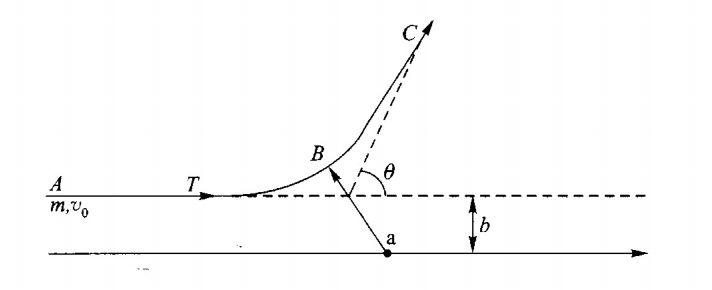
\includegraphics[width=0.45\textwidth]{1.png}
\\
\xiaowu\song 图~1\begin{minipage}[t]{75mm} \quad 散射角与瞄准距离的关系示意图.\\[-1mm]\wuhao
\end{minipage}
\end{center}
\subsection{微分散射截面}

有散射角与瞄准距离的关系式(2)可见,瞄准距离b增大,散射角$\theta$就小;反之,b小,$\theta$就大。只要瞄准距离b足够小,就可以足够大,这就解释了大角度散射的可能性。我们无法测量瞄准距离b,然而我们可以求出α粒子按瞄准距离的分布,根据这种分布就可以推出散射α粒子的角分布,而这个角分布是可以直接测量到的。

计算可以得到微分散射界面的公式为

\begin{equation}
	\frac{d \theta}{d \Omega} = (\frac{D}{2})^2 \frac{1}{\sin^2{(\theta/2)}} = (\frac{1}{4\pi\sigma_0})^2(\frac{Ze^2}{mv_0^2})^2\frac{1}{\sin^2{(\theta/2)}}
\end{equation}

试验过程中,探测器灵敏面积对靶所张的立体角为$\Delta\Omega$,则由卢瑟福散射公式得到某短时间内观察到的粒子数为
\begin{equation}
	N=(\frac{1}{4\pi\sigma_0})^2(\frac{Ze^2}{mv_0^2})^2nt\frac{\Delta\Omega}{\sin^4(\sigma/2)}T
\end{equation}

式中T为该时间内射到靶上的α粒子总数.由该式可见,在$\theta$方向上$\Delta\Omega$内所观测到$\alpha$粒子数N与散射靶的核电荷数Z、α粒子动能$1/2mv_0^2$及散射角$\theta$等因素都有关,其中N正比于$1/sin^4(\theta/2)$的关系是卢瑟福理论的最有力的验证。


\section{实验内容和结果}

本次的实验仪器如图所示:
\begin{center}
   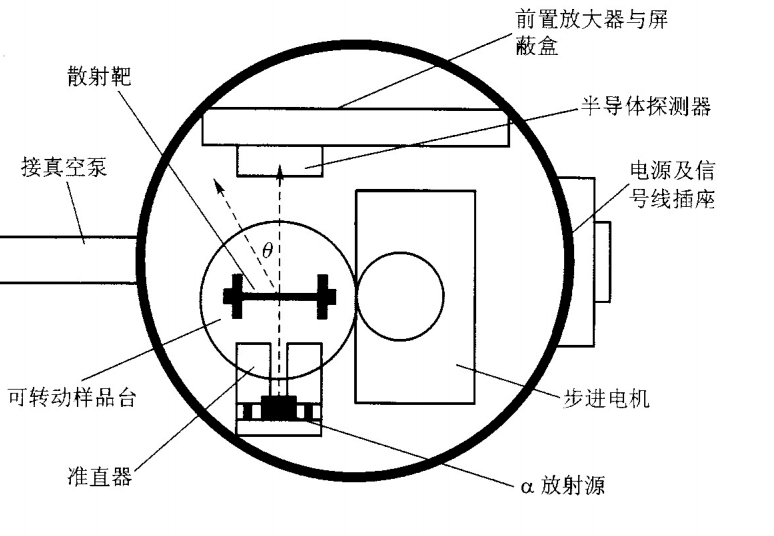
\includegraphics[width=0.45\textwidth]{jixie.png}
\\
\xiaowu\song 图~2\begin{minipage}[t]{75mm} \quad 实验装置中机械系统示意图。\\[-1mm]\wuhao
\end{minipage}
\end{center}
\begin{center}
   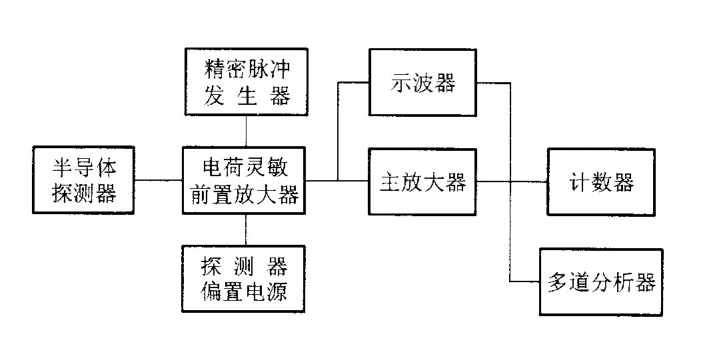
\includegraphics[width=0.45\textwidth]{yiqi.png}
\\
\xiaowu\song 图~3\begin{minipage}[t]{75mm} \quad 实验装置中探测系统示意图。\\[-1mm]\wuhao
\end{minipage}
\end{center}

按照图示连接好仪器后,首先是找出$\theta=0^{\degree}$的具体位置。确定方法是在$\theta = \pm10^{\degree}$附近测量,找到计数最大的位置。测量数据如下:

 \begin{center}
\bgliu
{\bf 表~1\quad
物理$0^{\degree}$角测量}\\[0.5mm]
\renewcommand{\arraystretch}{1.5}
\liuhao\song\rm
\newcolumntype{M}{>{\centering\arraybackslash}m{12mm} >{\centering\arraybackslash}m{12mm}>{\centering\arraybackslash}m{12mm} >{\centering\arraybackslash}m{12mm}}
\begin{tabular}{M}
\specialrule{0.1em}{1pt}{1pt}

位置/$^{\degree}$	&	计数	&	位置/$^{\degree}$	&	计数	\\
\midrule
-10	&	147	&	1	&	46937	\\
-9	&	597	&	2	&	46068	\\
-8	&	2684	&	3	&	46169	\\
-7	&	5383	&	4	&	43877	\\
-6	&	11191	&	5	&	42416	\\
-5	&	15771	&	6	&	38985	\\
-4	&	24345	&	7	&	36485	\\
-3	&	30642	&	8	&	31000	\\
-2	&	37596	&	9	&	25837	\\
-1	&	42380	&	10	&	17687	\\
0	&	45779	&	-	&	-	\\
\specialrule{0.1em}{3pt}{2pt}\\[-4mm]
\end{tabular}\\
\renewcommand{\arraystretch}{1.0}
\end{center}

\begin{center}
   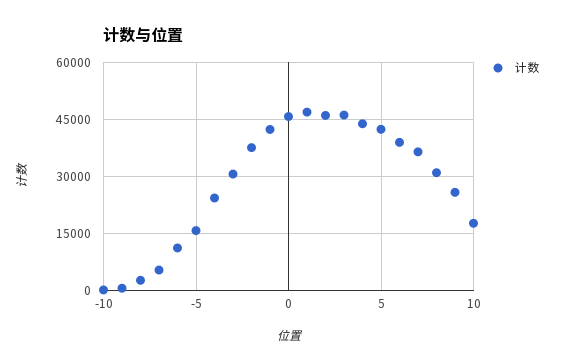
\includegraphics[width=0.45\textwidth]{2.png}
\\
\xiaowu\song 图~4\begin{minipage}[t]{75mm} \quad 计数随角度的变化曲线\\[-1mm]\wuhao
\end{minipage}
\end{center}
从数据中可以看出在$1^{\degree}$处为物理的$0^{\degree}$. 因此后续的计算就可以以此做矫正。(后续的角度数据都已修正)

而后测量在不同角度下的本底计数,数据如下:

 \begin{center}
\bgliu
{\bf 表~2\quad
本底计数}\\[0.5mm]
\renewcommand{\arraystretch}{1.5}
\liuhao\song\rm
\newcolumntype{M}{>{\centering\arraybackslash}m{20mm} >{\centering\arraybackslash}m{20mm}}
\begin{tabular}{M}
\specialrule{0.1em}{1pt}{1pt}

角度/$^{\degree}$	&	计数	\\
\midrule
20	&	62	\\
25	&	8	\\
30	&	4	\\
35	&	3	\\
40	&	1	\\
45	&	0	\\
50	&	0	\\
\specialrule{0.1em}{3pt}{2pt}\\[-4mm]
\end{tabular}\\
\renewcommand{\arraystretch}{1.0}
\end{center}

同理换上金箔靶,重新校正物理0点以及测量不同角度下的计数,数据如下:
 \begin{center}
\bgliu
{\bf 表~1\quad 加入Au箔靶后物理$0^{\degree}$角测量}\\[0.5mm]
\renewcommand{\arraystretch}{1.5}
\liuhao\song\rm
\newcolumntype{M}{>{\centering\arraybackslash}m{12mm} >{\centering\arraybackslash}m{12mm}>{\centering\arraybackslash}m{12mm} >{\centering\arraybackslash}m{12mm}}
\begin{tabular}{M}
\specialrule{0.1em}{1pt}{1pt}

位置/$^{\degree}$	&	计数	&	位置/$^{\degree}$	&	计数	\\
\midrule
-10	&	1637	&	1	&	32143	\\
-9	&	2876	&	2	&	31598	\\
-8	&	6278	&	3	&	31241	\\
-7	&	9344	&	4	&	29459	\\
-6	&	13448	&	5	&	27311	\\
-5	&	17206	&	6	&	23617	\\
-4	&	22086	&	7	&	19750	\\
-3	&	25427	&	8	&	15727	\\
-2	&	28665	&	9	&	11917	\\
-1	&	30007	&	10	&	7849	\\
0	&	31532	&	-	&	-	\\
\specialrule{0.1em}{3pt}{2pt}\\[-4mm]
\end{tabular}\\
\renewcommand{\arraystretch}{1.0}
\end{center}

 \begin{center}
\bgliu
{\bf 表~2\quad
卢瑟福散射计数,净计数为扣除本底计数后的结果}\\[0.5mm]
\renewcommand{\arraystretch}{1.5}
\liuhao\song\rm
\newcolumntype{M}{>{\centering\arraybackslash}m{12mm} >{\centering\arraybackslash}m{12mm}
>{\centering\arraybackslash}m{12mm}}
\begin{tabular}{M}
\specialrule{0.1em}{1pt}{1pt}

角度/$^{\degree}$	&	计数	&	净计数	\\
\midrule
20	&	1289	&	1227	\\
25	&	367	&	359	\\
30	&	161	&	157	\\
35	&	64	&	61	\\
40	&	52	&	51	\\
45	&	24	&	24	\\
50	&	18	&	18	\\
\specialrule{0.1em}{3pt}{2pt}\\[-4mm]
\end{tabular}\\
\renewcommand{\arraystretch}{1.0}
\end{center}

做出卢瑟福散射净计数和$1/\sin^4(\theta/2)$的关系图如下:

\begin{center}
   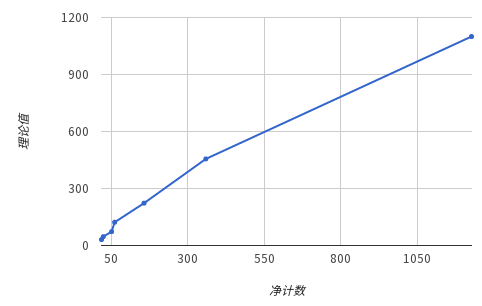
\includegraphics[width=0.45\textwidth]{3.png}
\\
\xiaowu\song 图~5\begin{minipage}[t]{75mm} \quad 卢瑟福散射公式的验证.\\[-1mm]\wuhao
\end{minipage}
\end{center}

从图中可以看出,散射$\alpha$计数N与$\frac{1}{\sin^4(\theta/2)}$基本呈线性关系,定性上验证了卢瑟福散射公式。

\section{结论}

本实验用$^{241}$Am的$\alpha$射线轰击金箔,通过测量散射$\alpha$粒子的计数,得到了计数N与角度函数$\frac{1}{\sin^4(\theta/2)}$的线性关系,在一定程度上验证了卢瑟福散射公式. 

\section{参考文献}

\noindent
[1] Peking Unviersity, Fudan University \ Nuclear Experment
\ Nuclear Publishing House, 1989 (in Chinese)

\noindent
 (北京大学,复旦大学.\ 原子核实验\ 原子能出版社,\ 1989)

\end{multicols}

\newpage

\clearpage
%\end{CJK*}
\end{document}

